% Report-only chapter: implementation detail the paper has no room for.
% Sources: docs/architecture/*.md, docs/protocols/watch-*.md, apps/watch/README.md,
% tools/label-trainer/README.md, docs/performance.md, crates/interaction-engine.
\chapter{Implementation}\label{ch:implementation}

This chapter describes how the system is built: the components and how they communicate, the watch application, the two watch transports, head tracking, the desktop application, the recording and labelling tools, model training and the run-time inference and interaction engine.

\section{Overall Architecture}

The system has four deployable parts (Table~\ref{tab:components}). The watch and the headphones only supply sensor data; training, inference, interaction decisions and every action take place on the desktop.

\begin{table}[htbp]
\centering
\caption{Deployable components.}\label{tab:components}
\begin{tabularx}{\linewidth}{@{}l>{\raggedright\arraybackslash}X>{\raggedright\arraybackslash}X@{}}
\toprule
\textbf{Component} & \textbf{Runs on} & \textbf{Ships as} \\
\midrule
Desktop application & macOS, Windows, Linux (development) & A Tauri bundle per operating system \\
Galaxy Watch application & Wear OS 3 or later & An APK installed over \texttt{adb} \\
Sony head-tracker provider & The same computer as the desktop application & Linked into the desktop binary on macOS and Windows; a separate process on Linux \\
Per-label trainer & A developer checkout & Not shipped; the desktop runs it through \texttt{uv} \\
\bottomrule
\end{tabularx}
\end{table}

The desktop backend is a Rust workspace split into crates with one job each: wire types (\texttt{protocol}), head tracking (\texttt{head-tracking}, \texttt{native-head-tracking}), watch transport (\texttt{watch-bridge}), feature extraction and model execution (\texttt{pinch-inference}, \texttt{label-inference}), interaction logic (\texttt{interaction-engine}) and native volume control (\texttt{volume-control}). The Tauri backend wires them together and talks to the React front end through Tauri events and commands. A second, transparent, always-on-top window shows the volume knob during a grab.

Several background tasks run in the backend. The watch event loop routes every incoming message. A watchdog checks every 200\,ms and force-releases any grab whose model data have been stale for 750\,ms. A time-sync task estimates the watch--desktop clock offset every 5\,s for display; it is never applied to samples. A dedicated thread applies volume changes, at most one write every 100\,ms, so that slow operating-system calls never block the event loop.

\section{Watch Application}

The watch application is a self-contained Kotlin project for Wear OS. It streams the rotation vector (as a quaternion), accelerometer and gyroscope readings, and on a Galaxy Watch4 or later, raw green, red and infrared PPG from the Samsung Health Sensor SDK. It also answers time-sync requests from the desktop immediately and sends a heartbeat once a second.

Battery life shaped much of the design. Sensors, PPG and the CPU wake lock run only while a desktop is connected and receiving. While the app is waiting for a desktop, it keeps a foreground service so that Samsung's background process freezer does not suspend it, but it releases every sensor and the wake lock. The standard off-body sensor pauses collection when the watch is taken off. PPG is sent whenever the SDK delivers samples, instead of on a fixed polling timer, and orientation messages are encoded with a plain string builder, which a JVM benchmark measured as eight times faster than the earlier JSON-object encoder (0.4 against 3.2\,µs per message).

\section{Watch--Desktop Transport}

The watch reaches the desktop over one of two transports, chosen on the watch and mirrored in the desktop settings. Exactly one is active at a time, and a failing transport reports its error instead of silently falling back to the other.

\paragraph{Bluetooth Low Energy (default).} The watch is the GATT peripheral and the desktop the central, because the Rust Bluetooth library (btleplug) supports only the central role and that role behaves the same on macOS, Windows and Linux. The service exposes a telemetry characteristic (watch to desktop, notify) and a command characteristic (desktop to watch, write with response). Both require an encrypted, bonded link, and the watch sends nothing until the user taps \emph{Trust this computer}. Over Bluetooth the desktop assigns the device identity from the peripheral it discovered, so a watch cannot choose or spoof its identity.

\paragraph{Wi-Fi.} The desktop runs a WebSocket server on port 8766, and the watch finds it through mDNS. This path is intended for a trusted local network only: it uses plain \texttt{ws://} with no encryption or authentication.

\paragraph{Message layer.} Both transports carry the same UTF-8 JSON envelopes with a type, protocol version, device identifier, sequence number, watch timestamp in nanoseconds and payload, and the desktop decodes both through one function. Timestamps use the watch's boot-relative clock. Freshness and dwell decisions are always made on the desktop's own monotonic clock.

\paragraph{Performance under load.} Profiling on real hardware showed the original Bluetooth path sending about 61 notifications a second, one per motion reading, with the send queue growing to 512 fragments (several seconds of delay) before it was dropped all at once. Batching motion readings into 100\,ms packets halved the notification rate to about 30 a second. The send queue now holds about 0.5\,s and drops the oldest unsent messages first. In a 15-minute streaming test, 20 messages (about 2\,s of data) were lost, mostly right after connecting. A fragment-size bug that made Android reject every PPG packet at a 517-byte MTU was also fixed.

Figure~\ref{fig:sensor-timing} shows the timing of the data that actually reached the desktop, measured from the watch timestamps in the 28 distinct recordings used to train and evaluate the hand-labelled model. Inertial samples arrive at a steady 100\,Hz: the median interval is 10.0\,ms and 99\% of intervals are within 10.1\,ms. PPG samples average 25\,Hz (median 40.0\,ms), but their individual intervals spread widely, up to 97\,ms. PPG reaches the app in batches from the Samsung sensor service, flushed up to ten times a second, and the timestamps within those batches are uneven. The model's fixed 20\,ms grid with zero-order hold absorbs this jitter, and no interval in either stream came near the 250\,ms gap that marks an input as unavailable.

\begin{figure}[htbp]
\centering
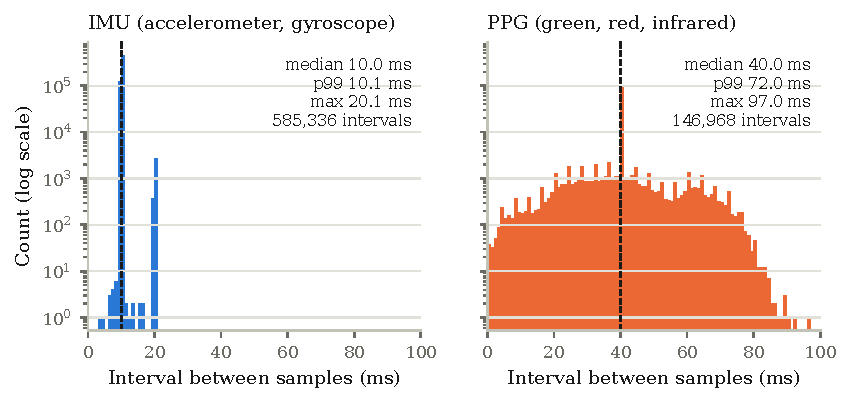
\includegraphics[width=\linewidth]{figures/sensor-timing.pdf}
\caption[Sample timing of the watch streams]{Intervals between consecutive samples, from watch timestamps in the 28 distinct recordings of the hand-labelled model. Dashed lines mark the nominal 10\,ms (IMU) and 40\,ms (PPG) periods. Log scale.}\label{fig:sensor-timing}
\end{figure}

\section{Head Tracking}

Head orientation comes from the motion sensors in Sony headphones. On macOS and Windows a native provider reads them in-process (through IOKit and IOBluetooth on macOS, HID and SetupAPI on Windows); on Linux, or when configured, an external command-line bridge sends JSON over loopback UDP to port 4243. Both feed the same provider interface.

Calibration stores a quaternion for the screen centre and for each target. At run time the engine measures the quaternion angular distance to each target and activates the nearest one after the head has stayed within 12° of it for 400\,ms. If the headphones reset their orientation reference, the calibration is invalidated and must be redone.

\section{Desktop Application}

The desktop application provides the live view of sensor streams, settings, calibration, the Recorder, Model Lab for training and managing models, and the inference mode switch (Off, Monitor, Live). A readiness indicator shows whether a pinch would be caught at that moment; after strong motion the CNN needs the wrist to be calm for about a second before it can catch a pinch again, and the indicator makes that visible.

All user state lives in the operating system's application directories: settings, recordings, datasets, the label catalogue, model bundles and the model registry. Writes that matter are atomic, and a corrupt registry file is reported as an error and left untouched instead of being replaced with an empty one.

\section{Recording and Labelling Tool}

The Recorder saves each session as an immutable bundle containing the raw sensor CSV, a metadata file and an annotations file. Bundles are staged and then renamed into place, so a crash never leaves a half-written recording, and they are never rewritten.

The Recorder can also save hand landmarks from the laptop camera. MediaPipe's Hand Landmarker runs inside the application's own web view, with its model and WebAssembly runtime served from the application's files; it finds 21 landmarks per hand in each frame. Only landmarks are saved, never images, and the application's content security policy blocks MediaPipe's attempt to send usage logs. To line the camera up with the watch, the Recorder logs pairs of watch timestamps and browser arrival times about every 200\,ms; on export, each camera frame is placed on the watch clock using the smallest arrival offset in the recording.

Exported datasets contain \texttt{ppg.csv} and \texttt{imu.csv}, plus the landmark and clock-sync files when a camera was used. Each sample keeps its original \texttt{label} column, and manual corrections go in a separate \texttt{manual\_label} column, following the rules described in Section~\ref{effective-label-semantics}.

\section{Model Training Pipeline}

Training runs offline in the Python \texttt{label-trainer}. The desktop decides everything that must be fixed in advance (which recordings train and which evaluate, never the same one, and what each label means: target, negative or left out) and passes it to the trainer in a specification file.

The trainer supports two model families:
\begin{itemize}
\item \textbf{ExtraTrees} (300 trees) on engineered features. The PPG-only version uses 1,701 features: each PPG channel is z-scored against the previous 1, 2 and 4\,s, its slope, curvature and jerk are estimated with a local cubic fit, and 21 statistics are taken over the last 8, 16 and 32 ticks of a 25\,Hz grid. The PPG+IMU version adds 1,032 motion features, for 2,733 in total. It fires about 0.9\,s after a pinch starts.
\item \textbf{CNN} on 450 inputs (nine channels by 50 ticks of a 50\,Hz grid), described in Section~\ref{models-and-learning-configuration}. It fires about 0.5\,s after a pinch starts.
\end{itemize}

The decision threshold is fitted on the training recordings, each scored by a model trained without it. The trainer then replays the model over every held-out recording through the same detection rule the runtime uses, and reports starts caught, delay and false activations per hour. The model is written as plain data (tree node arrays or JSON weights), never as executable code. A model that does not pass the checks for going live is still written, but as evaluation-only: the desktop can activate it in Monitor mode, where it only reports.

The same feature code exists twice, in Python for training and in Rust for live use. Shared test fixtures keep the two implementations numerically equal, so a model sees the same inputs in use as in training.

\section{Desktop Inference and Interaction Engine}

\paragraph{Model loading.} A model bundle is a manifest plus one model file. Before a model is loaded the runtime checks the manifest's schema, sources, feature names and order, input shape, window and file format; it checks that the file's SHA-256 matches the manifest, that the network's layers chain and its weights are finite, and that the model returns a probability on four constant test inputs. Only a registry version that is Active, and whose hash is the approved one, is loaded. The tree ensembles and the CNN are both evaluated in Rust, in-process, with no Python at run time.

\paragraph{Decision chain.} Each incoming PPG batch passes through an ordering check, a quality gate, a window check, fusion with recent orientation, feature extraction and the model, and the result goes to the gesture policy. Any stage that rejects a window forces a release of an open grab. Fusion rejects orientation older than 500\,ms, data from the wrong device and non-finite or out-of-order values.

\paragraph{Gesture policy.} The policy is a state machine that turns model events into the \texttt{VolumeGrab} and \texttt{VolumeRelease} intents, but only in Live mode and only for the intents explicitly bound to the active model. It ends a grab on a pinch-out, when the head leaves the target, on Escape, on stale or rejected data, on a mode change or when the model is replaced; a release that arrives together with a start wins.

\paragraph{Wrist mapper and volume writer.} At the start of a grab the mapper records the current wrist roll. Changes smaller than a 3° dead zone are ignored; beyond it, every 3° of roll moves the volume by one point, limited to 30 points a second and clamped to the valid range. A reading that implies rotation faster than 360°/s is treated as noise and ignored. Volume writes go to native back ends: Core Audio on Windows, the system volume on macOS, and \texttt{wpctl} or \texttt{pactl} on Linux. Each queued write is tagged with the grab it belongs to, so writes left over from a finished grab are discarded. Figure~\ref{fig:wrist-mapping} shows the mapping and the effect of the rate limit on a fast turn.

\begin{figure}[htbp]
\centering
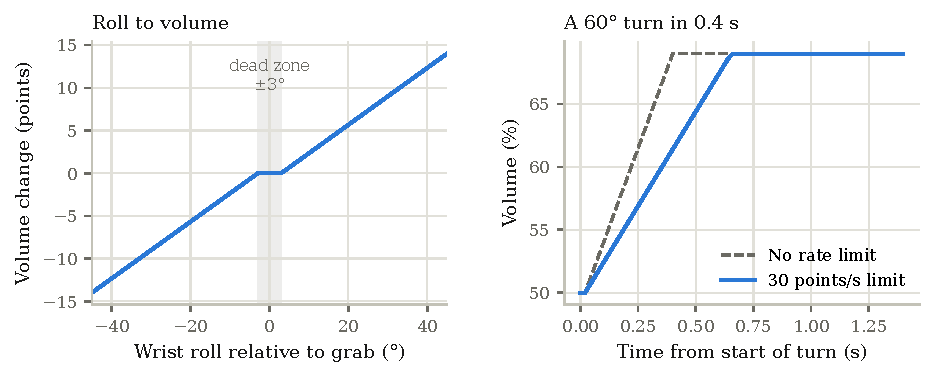
\includegraphics[width=\linewidth]{figures/wrist-mapping.pdf}
\caption[Wrist-roll to volume mapping]{Wrist-roll mapping with the default settings. Left: volume change against roll relative to the grab angle, with the $\pm3^\circ$ dead zone. Right: a simulated 60° turn made in 0.4\,s from volume 50, sampled at 50\,Hz; the 30 points/s limit stretches the change to about 0.65\,s. Computed from the interaction engine's default configuration.}\label{fig:wrist-mapping}
\end{figure}
